\documentclass[../Hovedrapport.tex]{subfiles}
\begin{document}
%%%%%%%%%%%%%%%%%%%%% døråbning %%%%%%%%%%%%%%%%%%%%%%%%
\section{Varmetilførsel ved åbning af dør (J.K. \& U.H.)}
    \label{sec:aabning_af_dor}
I følgende afsnit vil størrelsen af varmetilførslen ved åbning af køleskabsdøren bestemmes. Dette gøres for at få indsigt i, hvor stor en belastning dette har på køleskabet. 

Når døren åbnes sker der en udskiftning af luften inde i køleskabet. Denne luftudskiftning foregår som vist på figur \ref{fig:dør_luftstrøm}. Den kolde luft med en højere densitet vil strømme ud i bunden, mens den varme luft strømmer ind i toppen som følge af fri konvektion. Dette skyldes, at blæseren på fordamperen er tiltænkt at skulle være slukket under åbning af køleskabsdøren, da en tændt blæser vil give en tvungen strømning og hermed blæse alt den kolde luft ud af køleskabet. Den varmestrøm, systemet bliver tilført, vil blive beregnet ud fra fremgangsmåden beskrevet i \citep{koleteknik}, afsnit 10.3:
\begin{figure}[H]
    \centering
    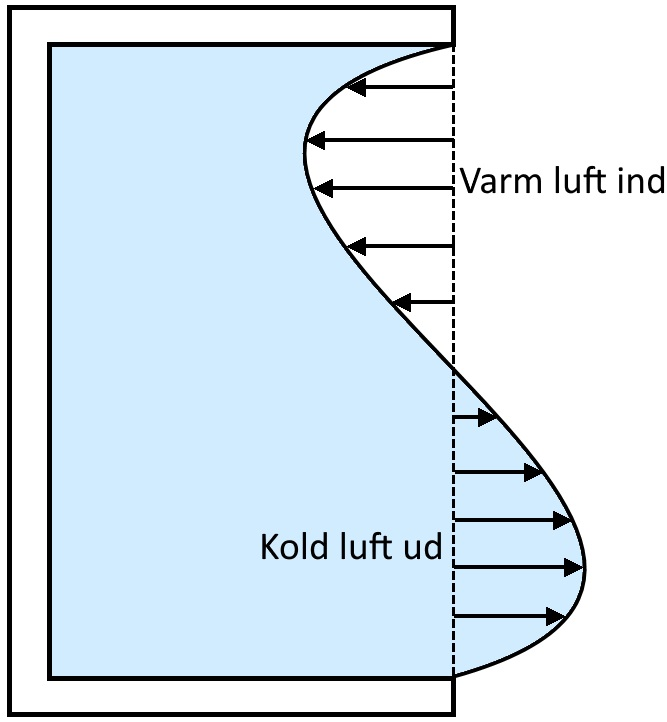
\includegraphics[width=0.3\textwidth]{Billeder/dør_luftstrøm.jpg}
    \caption{\textit{Luftudveksling ved døråbning}.}
    \label{fig:dør_luftstrøm}
\end{figure}

Varmestrømmen ind i køleskabet fås ved formlen:
\begin{equation}
\label{eq:varmestrøm_dør}
    \Phi_\text{dør} = q_\text{VL} \cdot \rho_\text{Lm} \cdot \left(h_\text{Lu} - h_\text{Li} \right)
\end{equation}
Hvori volumenstrømmen for luft, $q_\text{VL}$, defineres som:
\begin{equation}
    q_\text{VL} = \left( C_\text{inf} \cdot A_\text{dør} \cdot \sqrt{H_\text{dør}} \cdot \left( {\frac{\rho_\text{Li} - \rho_\text{Lu}}{\rho_\text{Li}}} \right)^{\frac{1}{2}} \cdot \left( \frac{2}{1+ {\left( {\frac{\rho_\text{Li}}{\rho_\text{Lu}}} \right)}^{\frac{1}{3}}} \right)^{\frac{2}{3}} \right) \cdot \eta_\text{Ls}
    \label{eq:volumenstrøm_dør}
\end{equation}
% jeg brugte 20 minutter på at skrive den skide formel...drengeren!

Forudbestemte konstanter til beregning af $\Phi_{\text{dør}}$ fremgår af tabel \ref{tab:doer_konstanter}:
\begin{table}[H]
\centering
\begin{tabular}{|c|c|c|}
\hline
\rowcolor[HTML]{C0C0C0} 
\multicolumn{3}{|c|}{\cellcolor[HTML]{C0C0C0}\textbf{Konstanter til beregning}} \\ \hline
\rowcolor[HTML]{EFEFEF} 
\textbf{Betegnelse} & \textbf{Beskrivelse}                                  & \textbf{Værdi}            \\ \hline
$t_\text{Lu}$       & Lufttemperatur uden for køleskab                      & \SI{30}{\celsius}         \\ \hline
$t_\text{Li}$       & Lufttemperatur inde i køleskab                        & \SI{4}{\celsius}          \\ \hline
$p_\text{L}$        & Trykket i luften                                      & \SI{1}{bar}           \\ \hline
$H_\text{dør}$      & Højden af døråbningen                                 & \SI{1,09}{m}              \\ \hline
$b_\text{dør}$      & Bredden af døråbningen                                & \SI{0,5}{m}               \\ \hline
$C_\text{inf}$      & Infiltrationskonstant                                 & \SI{0,692}{\sqrt{m}}/{s}    \\ \hline
$\eta_\text{Ls}$    & Virkningsgrad ved luftsluser (Sluser benyttes ikke)   & 1 \\ \hline
\end{tabular}
\caption{\textit{Konstanter til beregning af $\Phi_{\text{dør}}$}.}
\label{tab:doer_konstanter}
\end{table}
Indledningsvist bestemmes densiteter og entalpier for luften via \textit{EES} ud fra de ovenstående værdier. Disse fremgår af tabel \ref{tab:doer_konstanter_EES}:
\begin{table}[H]
\centering
\begin{tabular}{|c|c|c|c|}
\hline
\rowcolor[HTML]{C0C0C0} 
\multicolumn{4}{|c|}{\cellcolor[HTML]{C0C0C0}\textbf{Oplagsværdier fra EES}} \\ \hline
\rowcolor[HTML]{EFEFEF} 
\textbf{Betegnelse} & \textbf{Beskrivelse}      & \textbf{Baseret på}           & \textbf{Værdi}        \\ \hline
$\rho_\text{Lu}$    & Densitet - udvendig luft  & $t_\text{Lu}$, $p_\text{L}$   & \SI{1,150}{kg/m^3}    \\ \hline
$\rho_\text{Li}$    & Densitet - indvendig luft & $t_\text{Li}$, $p_\text{L}$   & \SI{1,258}{kg/m^3}    \\ \hline
$h_\text{Lu}$       & Entalpi - Udvendig luft   & $t_\text{Lu}$, $p_\text{L}$   & \SI{303,4}{kJ/kg}   \\ \hline
$h_\text{Li}$       & Entalpi - Indvendig luft  & $t_\text{Li}$, $p_\text{L}$   & \SI{277,3}{kJ/kg}   \\ \hline
\end{tabular}
\caption{\textit{Stofværdier fra EES}.}
\label{tab:doer_konstanter_EES}
\end{table}
Arealet af døråbningen beregnes:
\begin{equation*}
    A_\text{døråbning} = b_\text{døråbning} \cdot H_\text{døråbning} = \SI{0.55}{m^2}
\end{equation*}
Nu bestemmes luftens volumenstrøm ved åbning af køleskabsdøren ud fra formel \ref{eq:volumenstrøm_dør}:
\begin{equation*}
    q_\text{VL} = \SI{0,1129}{\frac{m^3}{s}}
\end{equation*}
Hvorefter varmestrømmen ved åbning af døren bestemmes med formel \ref{eq:varmestrøm_dør}
\begin{equation*}
    \Phi_\text{dør} = \SI{3554}{W}
\end{equation*}
Altså vil køleskabet opleve en varmestrøm på \SI{3554}{W}, når døren åbnes.
%--------------------------------------------------------------------------
\subsubsection*{Deldiskussion}
Denne udregningsmetode er generel for alle størrelser af kølerum. Derfor tages der ikke højde for elementer inde i køleskabet, som vil forhindre luftstrømmen ud af skabet. Der tages heller ikke højde for, at køleskabet indeholder en relativ lille volumen luft sammenlignet med et stort kølerum. Dermed vil en varmestrøm af denne størrelse, kun opleves meget kort tid efter åbning af døren. Det antages desuden i denne beregning, at luften er tør. Det vil i praksis kræve en større ydelse, når den nytilførte varme luft skal køles ned, da denne indeholder mere vand, som bliver kondenseret i forbindelse med nedkølingen.
\end{document}